%---------------------导言区---------------------------%
\documentclass[12pt,a4paper,UTF8]{ctexart}
	%10pt：正文字体为12pt，缺省为10pt；各层级字体大小会根据正文字体自动调整
	%a4paper：纸张大小a4；
	%UTF8：中文要求
\usepackage{geometry}%用于设置上下左右页边距
	\geometry{left=2.5cm,right=2.5cm,top=3.2cm,bottom=2.8cm}
\usepackage{xeCJK}
\usepackage{amsmath}
\usepackage{paralist}
\usepackage{enumerate}
\usepackage{booktabs}
\usepackage{multirow}
\usepackage{graphicx}
\usepackage{subfig}
\usepackage{setspace}
\usepackage{listings}
\usepackage{lastpage}
\usepackage{hyperref}
\usepackage{pdfpages}

%xeCJK：中文字体（如楷体，作者和机构需要用到）的设置
	%amsmath：数学公式
	%paralist，enumerate：自定义项目符号
	%booktabs：三线图，论文常用的表格风格
	%multirow：复杂表格
	%graphicx，float: 插入图片
	%subfig：并排排版图片、竖向排版图片
	%setspace：设置行间距等功能
	\setlength{\parindent}{2em}%正文首行缩进两个汉字
	%listings:用于排版各种代码；比如matlab的代码
	\lstset{language=Matlab}%matlab代码
	%lastpage:获取总页数;
	%hyperref:超链接,和lastpage搭配.
\usepackage{fancyhdr}
	%fancyhdr：一个很强大的宏包，用于自定义设计页面风格并命名以供调用。
	\pagestyle{fancy}
	\rhead{核磁共振稳态吸收}
	\lhead{近代物理实验~~~实验报告}
	\cfoot{Page \thepage/\pageref{LastPage}}  %当前页\总页数
	\rfoot{\today}
		%分别是右页眉、左页眉、中页脚、右页脚
	\renewcommand{\headrulewidth}{0.4pt}
	\renewcommand{\theenumi}{(\arabic{enumi})}

%%%%%%%%%%%%%%%%%%%%%%%%%%%%%%%%%%%%%%%%%%%%%%%%%%%%%%%%%%
%%%%%%%%%%%%%%%%%%%%%%%%%正文开始%%%%%%%%%%%%%%%%%%%%%%%%%%
%%%%%%%%%%%%%%%%%%%%%%%%%%%%%%%%%%%%%%%%%%%%%%%%%%%%%%%%%%

\begin{document}

%%begin-------------------标题与信息-----------------------%%

%%标题
\begin{center}
\LARGE\textbf{核磁共振稳态吸收}
\end{center}

%%信息
\begin{doublespacing}
	%doublespacing：手动两倍行距
	\begin{tabular}{lr}
	 & \\
	 {实验人姓名：徐殊行~23343071} & {合作者姓名：王志超~23343062}\\
	 {实验时间：2025年6月13日/20日} & {室温：27$^{\circ}$C~相对湿度：88\%}
	
	\end{tabular}
\end{doublespacing}

%%-------------------中英文摘要-----------------------%%
\begin{abstract}
    \noindent 本文介绍了连续波核磁共振稳态吸收实验的原理、操作与分析方法。
    通过将含氢样品置于高均匀度静磁场中，并叠加频率可调的射频场，观察吸收信号随频率或磁场的变化曲线；
    在此基础上，利用布洛赫方程的稳态解分析信号峰值与线宽，并结合玻尔兹曼分布与弛豫动力学，定量计算氢核的旋磁比、朗德因子、核磁矩及横向弛豫时间。
    实验结果验证了核磁共振频率与静磁场成正比关系，谱线宽度主要由横向弛豫时间 $T_{2}$决定。
    该实验强化了对核磁共振量子—经典模型的理解，并培养对高灵敏信号检测与参数提取的实践能力。\cite{wu1999modern,zheng1988modern,wu1999modern2,lin1999course}

    \noindent \textbf{关键词：} 核磁共振；稳态吸收；布洛赫方程；弛豫时间；拉莫尔进动
		
\end{abstract}
	
\renewcommand{\abstractname}{Abstract}

\begin{abstract}
    \noindent This work presents the steady-state absorption experiment of continuous-wave Nuclear Magnetic Resonance (NMR).
    An H-containing sample is placed in a high-uniformity static magnetic field, with a tunable RF field superimposed.
    Absorption signals are recorded by either frequency sweep or field sweep methods.
    Using the steady-state solution of the Bloch equations, the resonance peak amplitude and linewidth are analyzed in conjunction with Boltzmann distribution and relaxation dynamics.
    Quantitative determination of the proton gyromagnetic ratio \(\gamma\), nuclear \(g\)-factor, nuclear magnetic moment \(\mu_N\), and transverse relaxation time \(T_2\) is achieved from the measured spectra.
    The results confirm that the resonance frequency scales linearly with the static field strength and that the linewidth is predominantly governed by \(T_2\).
    This experiment reinforces the dual quantum–classical picture of NMR and hones practical skills in high-sensitivity signal detection and parameter extraction.
   
	\noindent \textbf{Keywords: } Nuclear Magnetic Resonance; Steady-State Absorption; Bloch Equations; Relaxation Time; Larmor Precession
\end{abstract}

%%-------------------正文部分-----------------------%%

\subsection*{【实验目的】}
\begin{enumerate}[(1)]
    \item 了解核磁共振的基本原理，掌握核磁共振现象的产生条件；
    \item 利用核磁共振方法测量样品的磁旋比γ、核朗德因子g和原子核磁矩μ；
    \item 了解利用核磁共振精确测量磁场强度的方法；
    \item 掌握核磁共振实验仪器的使用方法和数据处理技术。
\end{enumerate}

\subsection*{【实验原理】}
\subsubsection*{1. 核磁共振的量子力学描述（单个核的磁共振）}
原子核自旋量子数 \(I\) 决定角动量大小：
\[
|\mathbf{I}| = \sqrt{I(I+1)}\,\hbar.
\]
磁矩与角动量关系：
\[
\boldsymbol{\mu} = \gamma\,\mathbf{I}, 
\quad \gamma = g_N\frac{e}{2m_p},
\]
其中 \(g_N\) 为核朗德因子，\(\mu_N=\tfrac{e\hbar}{2m_p}\) 为核磁子。  

在静磁场 \(\mathbf{B}_0\) 中，磁量子数 \(m=-I,\dots,I\) 对应能级：
\[
E_m = -m\,g_N\mu_N\,B_0.
\]
相邻两能级差
\[
\Delta E = g_N\mu_N\,B_0,
\]
满足共振条件
\[
h\nu_0 = \Delta E
\;\Longrightarrow\;
\nu_0 = \frac{g_N\mu_N}{h}\,B_0,
\quad
\omega_0 = \gamma\,B_0.
\]

\subsubsection*{2. 核磁共振的宏观理论描述（多个核的磁共振）}
\paragraph{（1）拉莫尔进动}
将宏观磁化强度 \(\mathbf{M}\) 视作矢量和，单个磁矩进动方程：
\[
\frac{d\boldsymbol{\mu}}{dt} = \gamma\,\boldsymbol{\mu}\times\mathbf{B}_0
\;\Longrightarrow\;
\omega_0=\gamma B_0.
\]
加射频场 \(\mathbf{B}_1\perp\mathbf{B}_0\)，仅当 \(\omega=\omega_0\) 时磁矩能量被有效吸收，共振发生。

\paragraph{（2）热平衡与净吸收}
大量核在热平衡下遵从玻尔兹曼分布：
\[
\frac{N_2}{N_1}
=\exp\Bigl(-\frac{\Delta E}{k_BT}\Bigr)
\approx1-\frac{g_N\mu_NB_0}{k_BT},
\]
低能级核略多，产生净吸收信号，幅度微弱，需高灵敏度检测。

\paragraph{（3）布洛赫方程与稳态吸收}
宏观磁化 \(\mathbf{M}\) 在外场与弛豫作用下演化由布洛赫方程给出：
\[
\frac{d\mathbf{M}}{dt}
=\gamma\,\mathbf{M}\times\mathbf{B}
-\frac{M_x\hat{\mathbf{i}}+M_y\hat{\mathbf{j}}}{T_2}
-\frac{M_z-M_0}{T_1}\,\hat{\mathbf{k}},
\]
其中
\(\mathbf{B}=\mathbf{B}_0+\mathbf{B}_1\cos(\omega t)\),
\(T_1\) 为纵向弛豫时间，\(T_2\) 为横向弛豫时间。

在与射频场同频的旋转坐标系中求稳态解，可得吸收分量 \(v(\omega)\)：
\[
v(\omega)=\frac{\gamma B_1 T_2\,M_0}
{1 + T_2^2(\omega_0-\omega)^2 + \gamma^2B_1^2T_1T_2},
\]
共振峰值出现在 \(\omega=\omega_0\)，半高宽约为
\(\Delta\omega_{1/2}\approx1/T_2\)，由 \(T_2\) 决定谱线宽度。

\subsection*{【实验仪器】}
\begin{table}[h!]
	\centering
	\begin{tabular}{|p{5cm} p{4cm} p{5cm}|}
		\hline
		仪器名称 & 型号 & 参数 \\
		\hline\hline
		连续波核磁共振仪 & FD-CNMR-B &  \\
		示波器 & Tek MDO4034C & 350MHz~2.5GHz \\
		\hline		
	\end{tabular}
	\caption{实验仪器及参数}
	\label{tab:instruments}
\end{table}

实验中还用到了各种浓度的硫酸铜水溶液，以及氢氟酸，丙三醇，硫酸镉水溶液，纯水等样品，在图\ref{fig:samples}中给出了这些样品的共振信号。
\begin{figure}[h!]
    \centering
    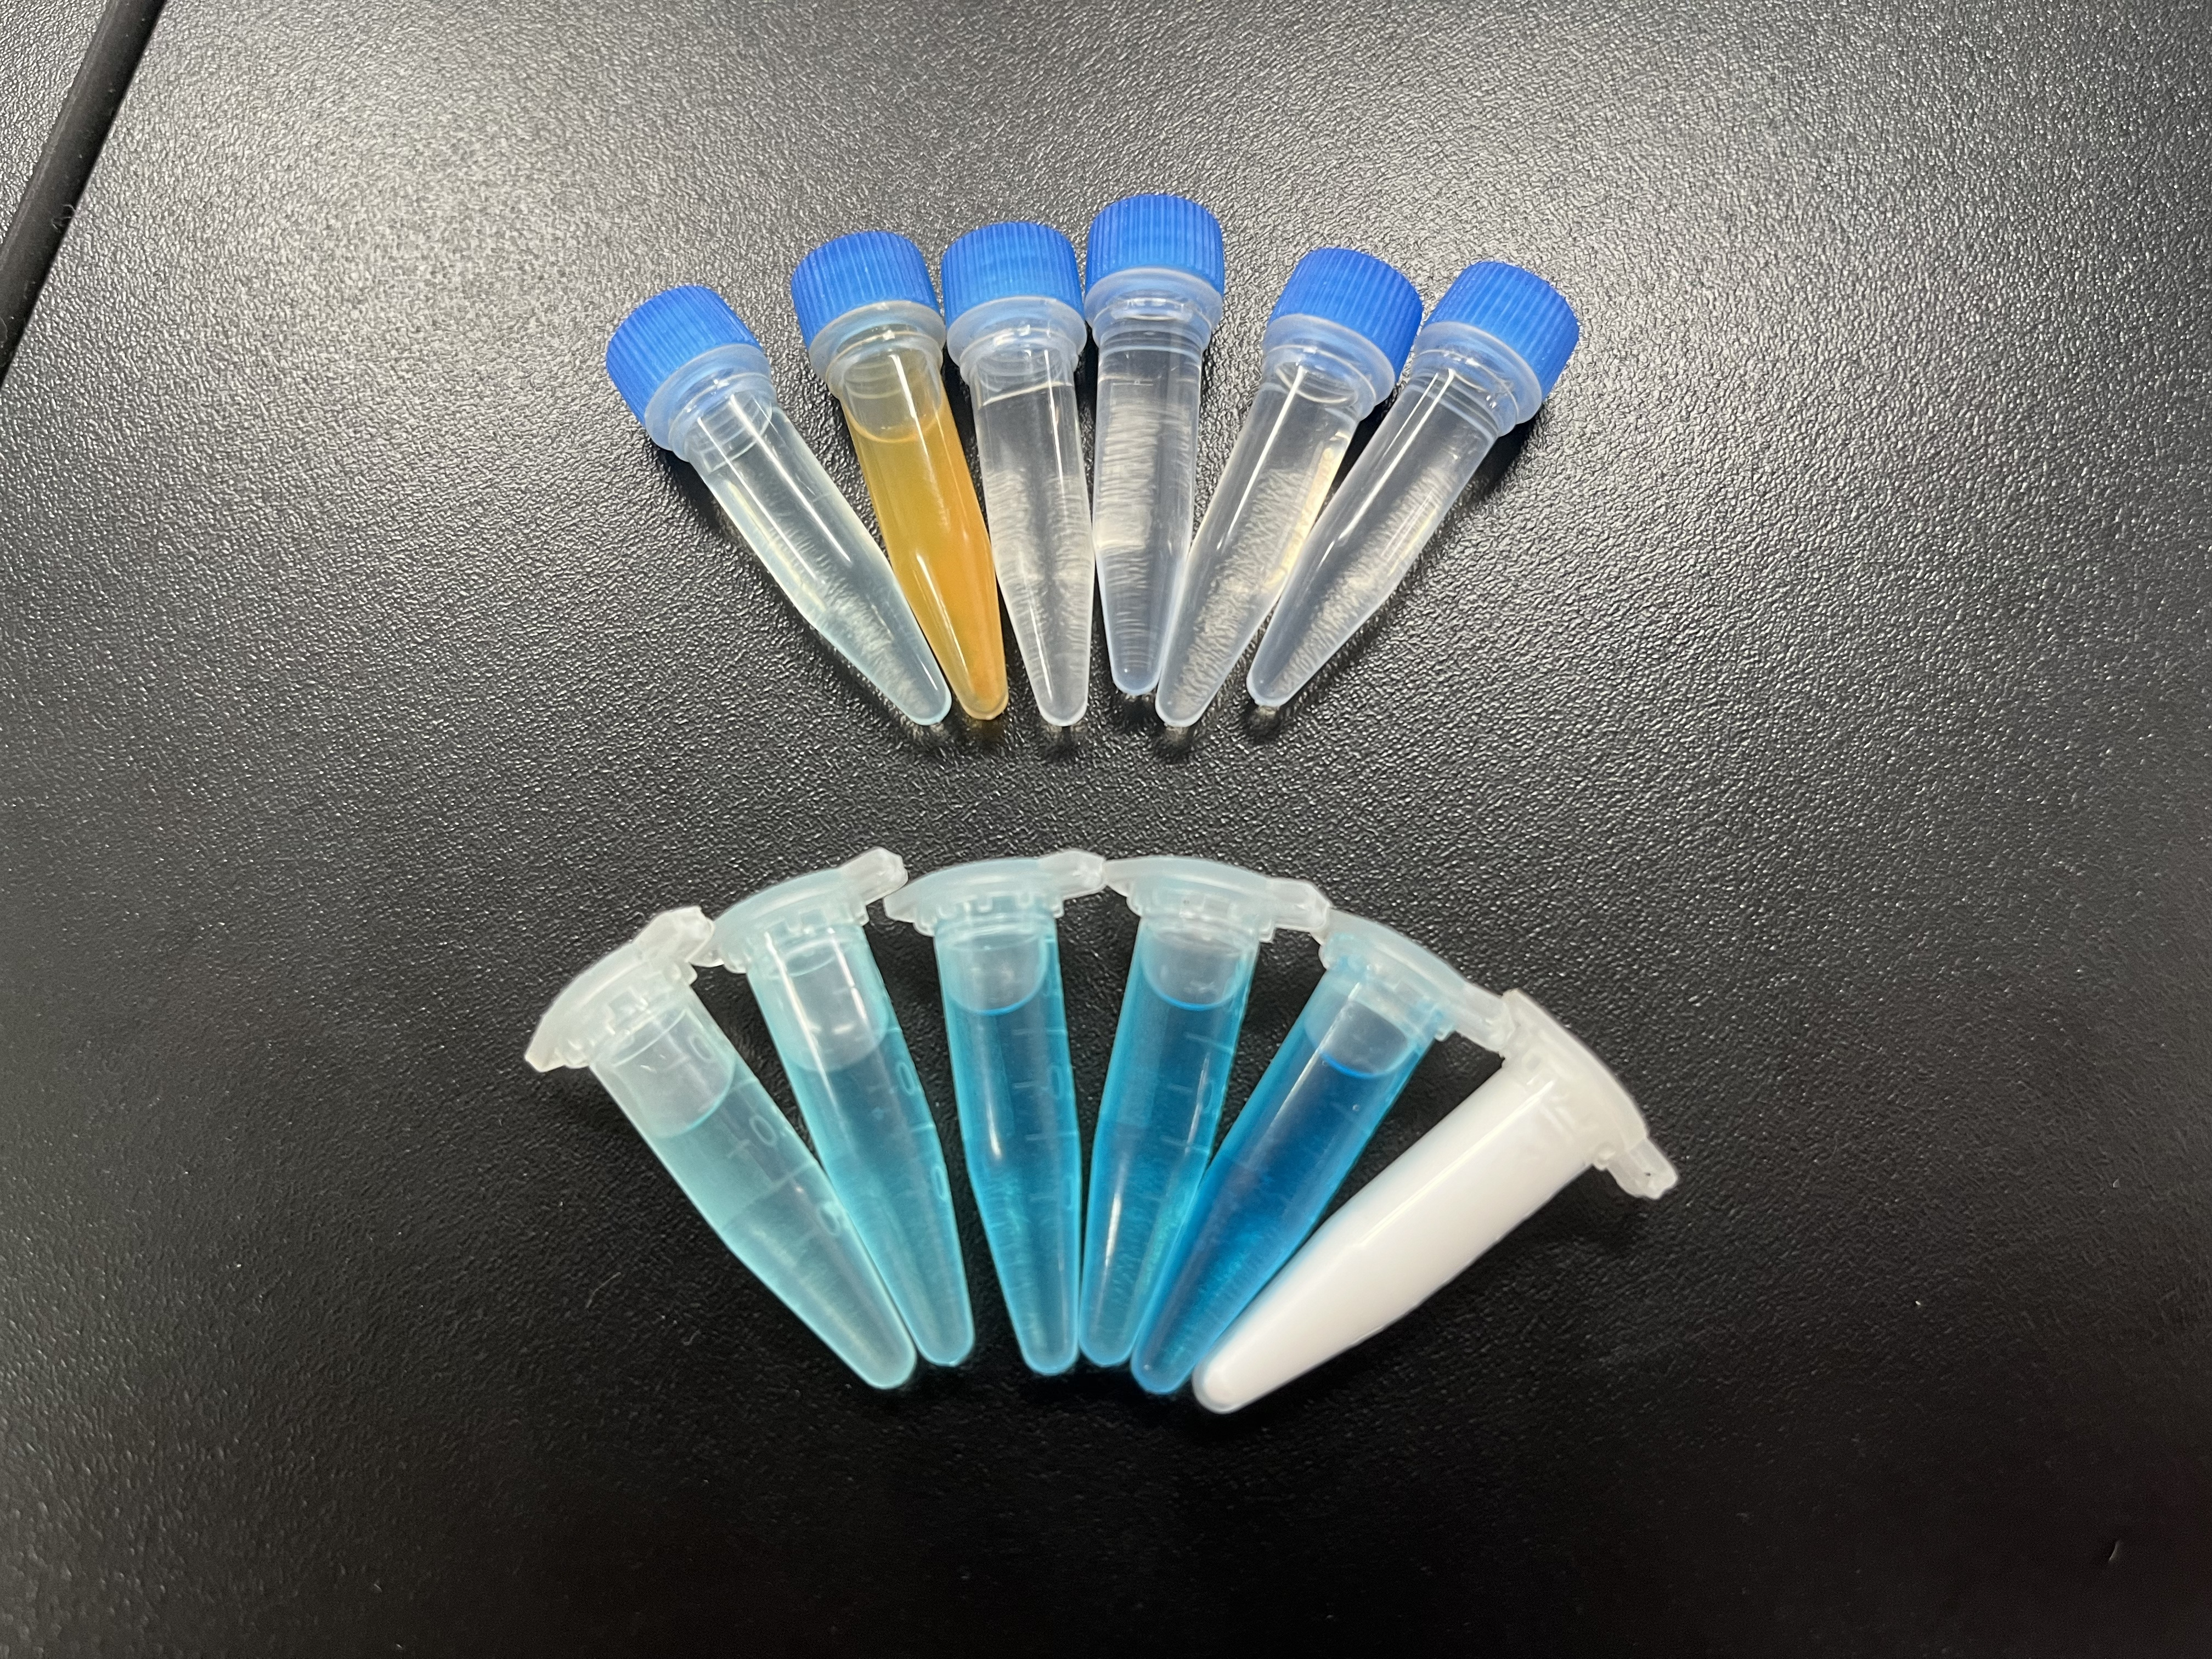
\includegraphics[width=0.45\textwidth]{samples.jpg}
    \caption{不同样品的共振信号}
    \label{fig:samples}
\end{figure}

\subsection*{【实验内容】}
\begin{enumerate}[(1)]
    \item 理解实验物理原理和实验技术原理；了解实验系统各仪器的功能及使用方法。
    \item 确认连续波核磁共振实验仪、频率计和示波器等实验仪器之间的连接：
    \begin{enumerate}[a]
        \item 将连续波核磁共振实验仪的输出信号连接到示波器的CH1通道
        \item 将频率计连接到连续波核磁共振实验仪的频率输出端口
        \item 确保所有仪器正确接地
    \end{enumerate}
    \item 调节实验仪样品杆的位置使被测样品靠近磁场中心。
    \item 调节实验仪"射频幅度"旋钮，使"射频幅度"处于$3.5-5.0\mathrm{V}$之间。
    \item 调节实验仪边限振荡器"频率粗调"和"频率细调"旋钮，观察示波器信号变化。
    \item 观察并分析共振尾波的物理过程：
    \begin{enumerate}[a]
        \item 记录尾波振荡频率的变化规律
        \item 分析尾波幅值衰减的物理机制
    \end{enumerate}
    \item 改变扫描电源的"扫描幅度"，观察并记录示波器信号的变化情况，分析扫描幅度对共振信号的影响。
    \item 改变样品在磁场中的位置，观察并记录示波器信号的变化情况，分析样品位置对共振信号的影响。
    \item 记录样品所在处的磁场强度及对应的共振频率，分析实验结果。
    \item 查阅文献资料，从理论上理解（分析）课堂上所观察到的实验现象。
    \item 重复步骤（7）和（8）实验内容，使用数字存储示波器记录实验结果。
    \item 观察记录不同浓度硫酸铜水溶液的实验结果，并（半）定量分析其物理规律。
    \item 收拾实验仪器，整理实验数据，实验完毕。
\end{enumerate}

\subsection*{【实验过程和数据处分析处理】}
首先我们按照实验要求和说明书上的步骤正确连接好各个仪器，随后可以开始进行实验。

\subsubsection*{调节共振信号}
首先我们需要调节实验样品的位置，使其靠近磁场中心，尽量处在匀强磁场区域。
随后我们将硫酸铜水溶液放置在样品杆上，然后反复调节射频幅度和频率，观察示波器上的信号变化，尽量获得效果更好的共振信号。

在实验过程中我们发现射频幅度在$4.17~4.18\mathrm{V}$时能够获得效果较好的共振信号。
此时再用高斯计测量样品位置的磁场强度，$B = 431.1.5 \mathrm{mT} $

在后面的实验中我们尽量保持这些参数不变，进行不同样品共振信号的观察和共振频率的测量。

\subsubsection*{测量不同样品的共振频率}
实验室提供了六种不同的样品，如表\ref{tab:samples}所示
\begin{table}[h!]
	\centering
	\begin{tabular}{|c|c|}
		\hline
		样品编号 & 样品内容 \\
		\hline\hline
		1 & 硫酸铜水溶液 \\
		2 & 三氯化铁溶液 \\
		3 & 氢氟酸 \\
		4 & 丙三醇 \\
		5 & 纯水 \\
		6 & 硫酸镉水溶液 \\
		\hline		
	\end{tabular}
	\caption{实验样品列表}
	\label{tab:samples}
\end{table}

\begin{figure}[h!]
    \centering
    \begin{minipage}[b]{0.48\textwidth}
        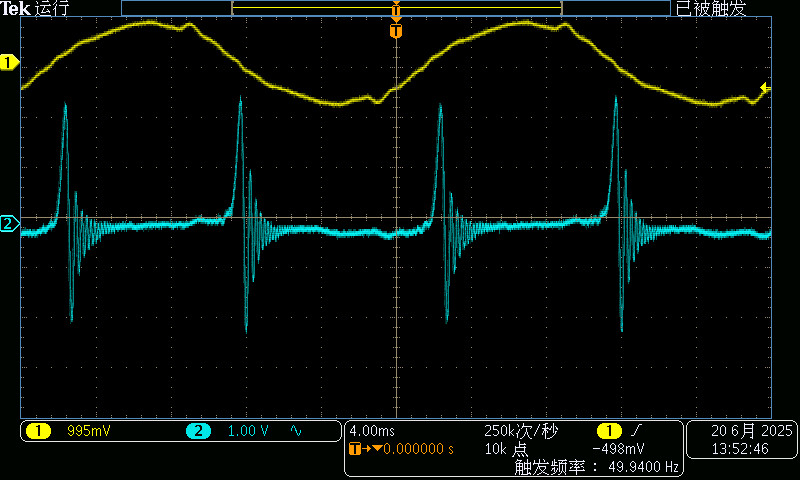
\includegraphics[width=\textwidth]{tek00002.png}
        \caption{硫酸铜水溶液}
    \end{minipage}
    \hfill
    \begin{minipage}[b]{0.48\textwidth}
        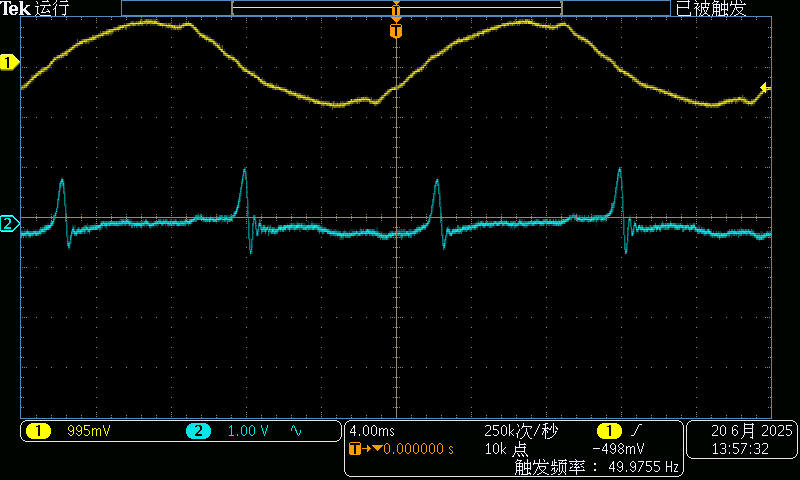
\includegraphics[width=\textwidth]{tek00003.png}
        \caption{三氯化铁溶液}
    \end{minipage}
        
    \begin{minipage}[b]{0.48\textwidth}
        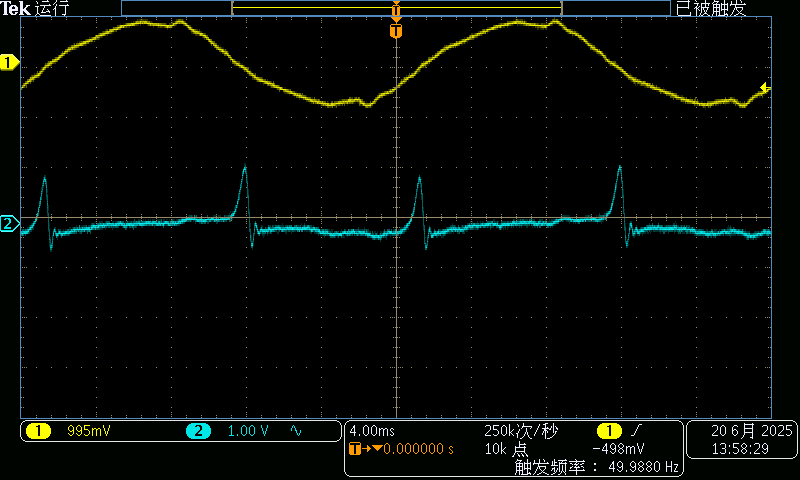
\includegraphics[width=\textwidth]{tek00004.png}
        \caption{氢氟酸}
    \end{minipage}
    \hfill
    \begin{minipage}[b]{0.48\textwidth}
        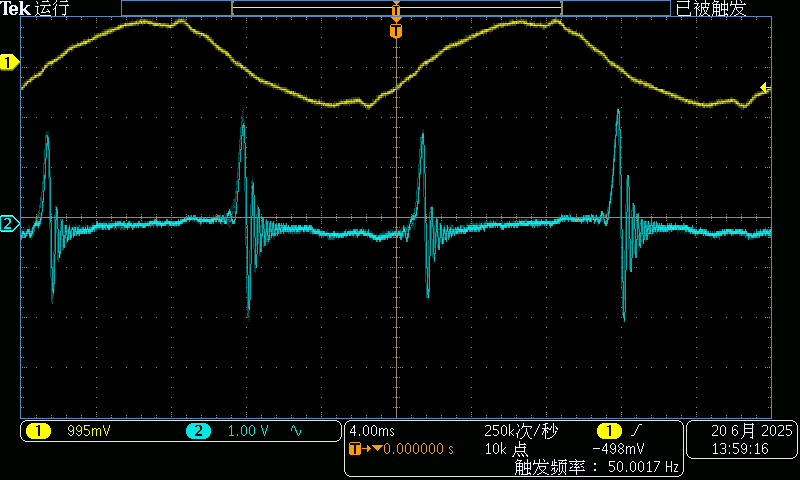
\includegraphics[width=\textwidth]{tek00005.png}
        \caption{丙三醇}
    \end{minipage}
    
    \begin{minipage}[b]{0.48\textwidth}
        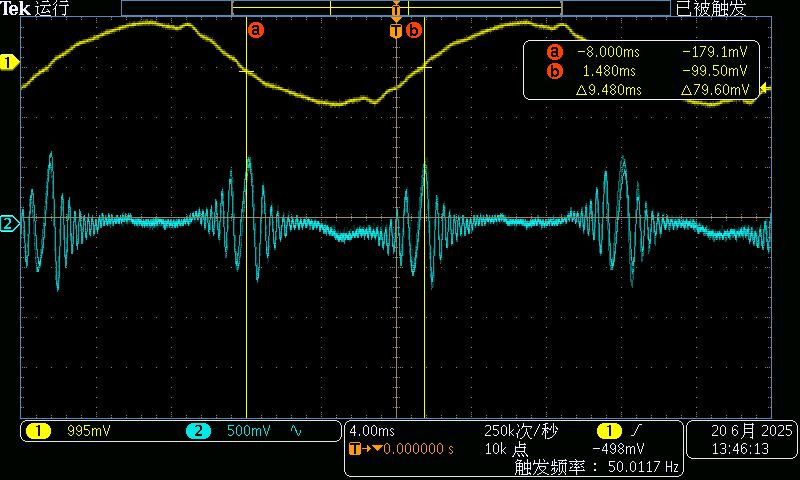
\includegraphics[width=\textwidth]{tek00000.png}
        \caption{纯水}
    \end{minipage}
    \hfill
    \begin{minipage}[b]{0.48\textwidth}
        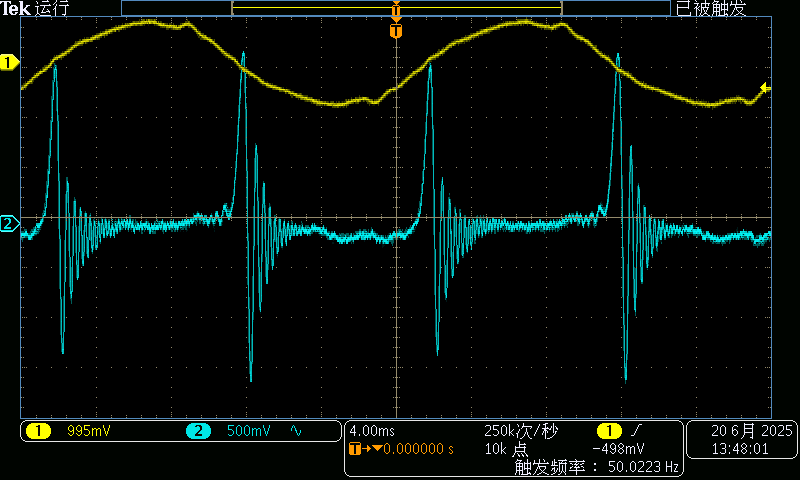
\includegraphics[width=\textwidth]{tek00001.png}
        \caption{硫酸镉水溶液}
    \end{minipage}
    \caption{不同样品的共振信号}
    \label{fig:samples}
\end{figure}

其中比较有趣的是纯水样品的共振信号，从图中可以看出，其共振信号波形表现出“拍”的形状，图\ref{fig:purewater}展示了水的共振吸收信号的更多细节。
这在一定程度上说明，纯水样品的共振信号可能是某两种频率十分相近的信号的叠加。

\begin{figure}[h!]
    \centering
    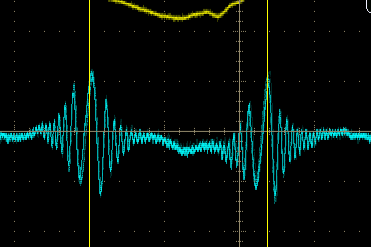
\includegraphics[width=0.45\textwidth]{tek00000_detail.png}
    \caption{纯水样品的共振信号}
    \label{fig:purewater}
\end{figure}

我们尝试解释这种“拍”的出现原因。
第一种解释是由于水分子种有两个氢原子，理论上来说二者的共振频率应当完全相同，
但是由于水分子的化学状态不同，两个氢原子核的共振频率可能有些许差异，这就有可能导致实验中观察到“拍”的现象出现。

另一种解释是水分子的弛豫时间较长，在前一个共振信号弛豫衰减的过程中频率略有下降，
而弛豫时间较长导致下一个共振信号会和前一个频率已经衰减的共振信号发生干涉，这两个信号的频率也十分相近，有可能导致实验上观察到“拍”的现象出现。

根据我们查阅的文献，第二种解释更加合理，而且实验室给出的参考数据指出，纯水样品的弛豫时间有$2s$左右，这与我们提出的解释相符。

\clearpage
\subsubsection*{共振频率和弛豫时间的测量}
承接上面的实验，我们同时记录下来每个样品出现共振的时候，频率计的读数，并利用示波器的测量功能测出每个样品的共振弛豫时间。
二者的结果如表\ref{tab:resonance}所示。

\begin{table}[h!]
    \centering
    \begin{tabular}{|c|c|c|}
        \hline
        样品编号 & 共振频率 (MHz) & 弛豫时间 (ms) \\
        \hline\hline
        1 & 20.5637 & 1.570 \\
        2 & 20.5640 & 2.040 \\
        3 & 20.5627 & 3.720 \\
        4 & 20.5640 & 3.940 \\
        5 & 20.5645 & 3.580 \\
        6 & 20.5657 & 4.900 \\
        \hline
    \end{tabular}
    \caption{不同样品的共振频率和弛豫时间}
    \label{tab:resonance}
\end{table}

需要指出的是，上面表格中纯水的弛豫时间与参考数据不符，是因为我们把“拍”信号的衰减时间作为是弛豫时间来测量。
但是纯水的弛豫时间应当在$2s$左右，这可能超过了我们示波器能观察的范围。

\subsubsection*{扫场强度对尾波的影响}
我们在实验中还测量了扫场强度对尾波的影响，我们使用硫酸铜的水溶液作为样品，在调节出较好的共振信号之后，
我们逐渐增加扫场强度，观察示波器上的信号变化，主要观察共振信号的弛豫尾波长度。
实验结果如图\ref{fig:sweep}所示，图中随着序号增大扫场幅度逐渐增大。

\begin{figure}[h!]
    \centering
    % 第一排：三张图片并排
    \begin{minipage}[b]{0.32\textwidth}
        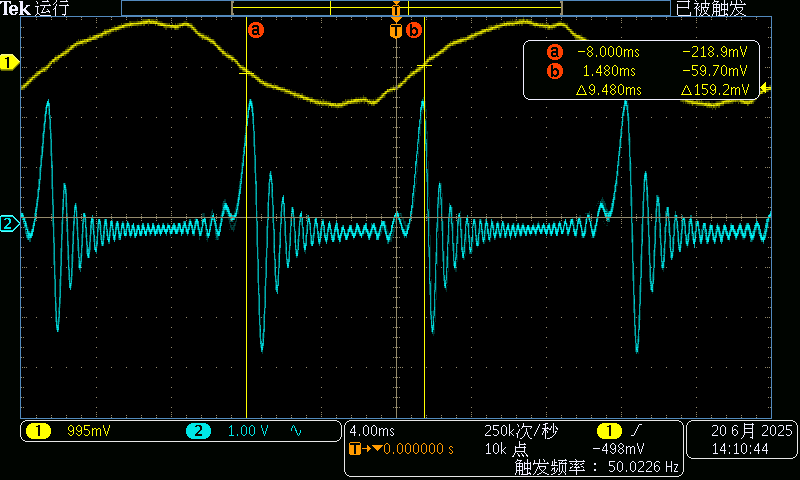
\includegraphics[width=\textwidth]{tek0000.png}
        \caption*{扫场电压1}
    \end{minipage}
    \hfill
    \begin{minipage}[b]{0.32\textwidth}
        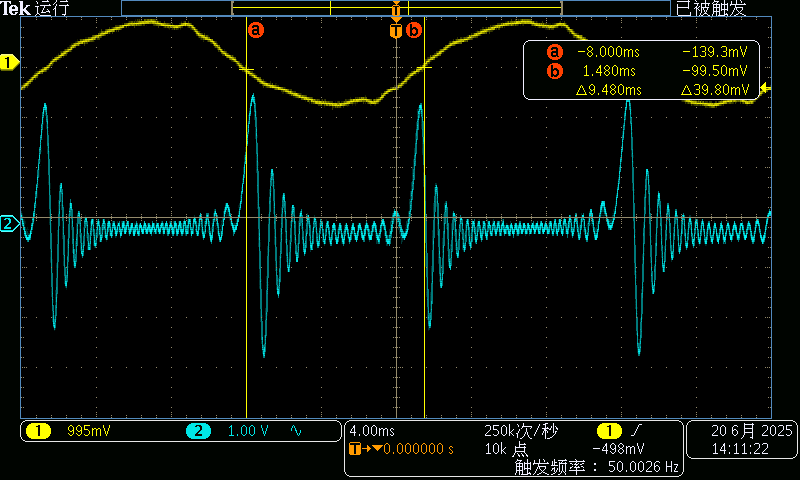
\includegraphics[width=\textwidth]{tek0001.png}
        \caption*{扫场电压2}
    \end{minipage}
    \hfill
    \begin{minipage}[b]{0.32\textwidth}
        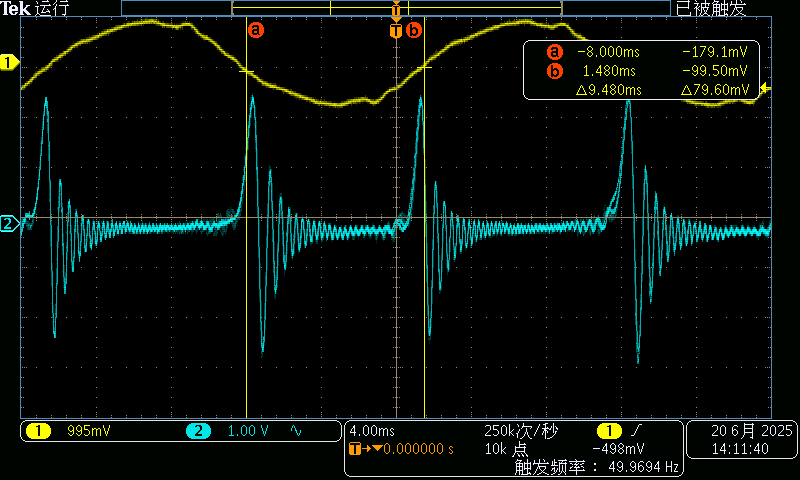
\includegraphics[width=\textwidth]{tek0002.png}
        \caption*{扫场电压3}
    \end{minipage}
    % 第二排：三张图片并排
    \begin{minipage}[b]{0.32\textwidth}
        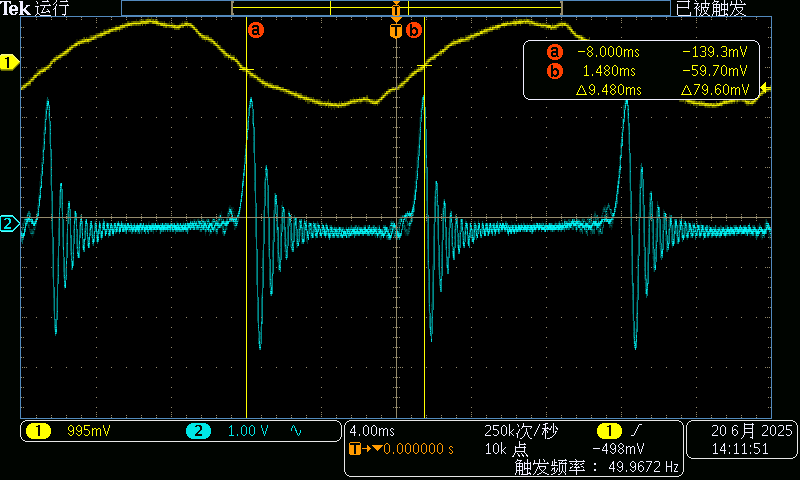
\includegraphics[width=\textwidth]{tek0003.png}
        \caption*{扫场电压4}
    \end{minipage}
    \hfill
    \begin{minipage}[b]{0.32\textwidth}
        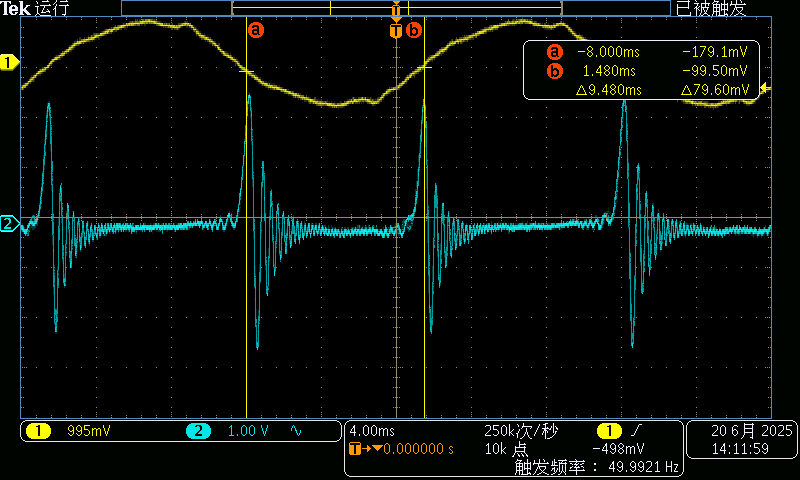
\includegraphics[width=\textwidth]{tek0004.png}
        \caption*{扫场电压5}
    \end{minipage}
    \hfill
    \begin{minipage}[b]{0.32\textwidth}
        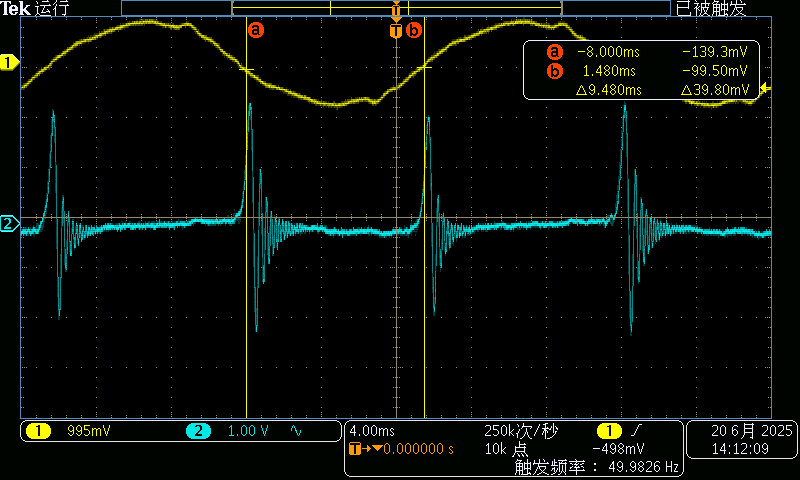
\includegraphics[width=\textwidth]{tek0005.png}
        \caption*{扫场电压6}
    \end{minipage}
    % 第三排：两张图片并排
    \begin{minipage}[b]{0.48\textwidth}
        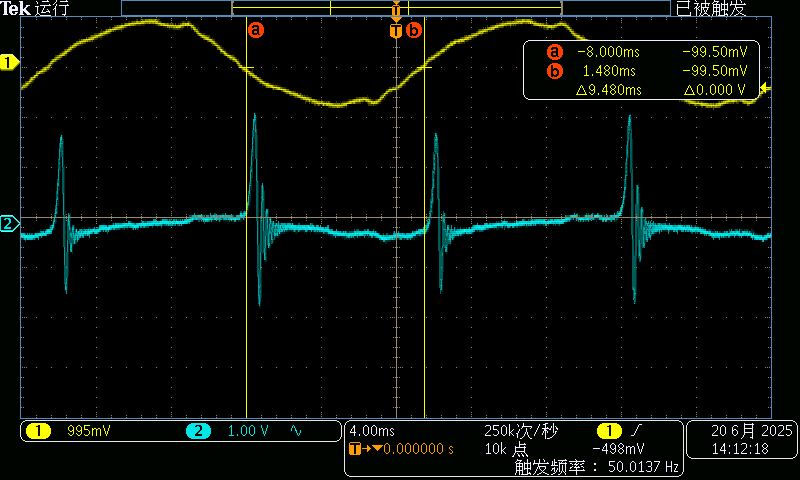
\includegraphics[width=\textwidth]{tek0006.png}
        \caption*{扫场电压7}
    \end{minipage}
    \hfill
    \begin{minipage}[b]{0.48\textwidth}
        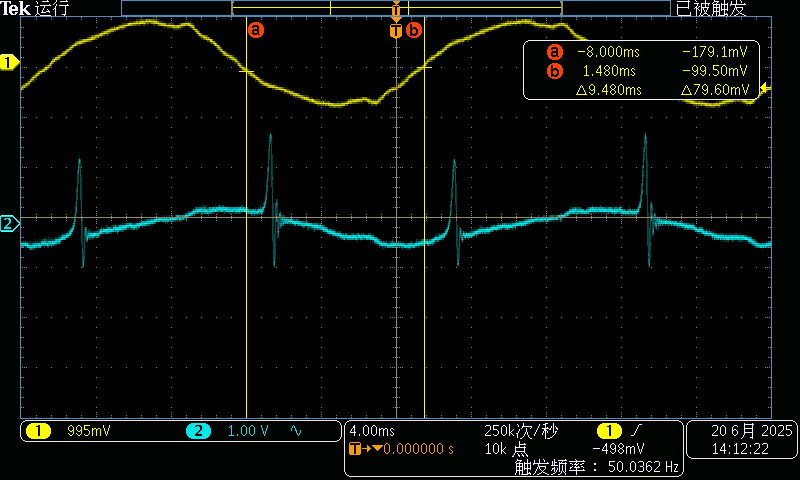
\includegraphics[width=\textwidth]{tek0007.png}
        \caption*{扫场电压8}
    \end{minipage}
    \caption{扫场强度对尾波的影响}
    \label{fig:sweep}
\end{figure}

观察上示波器上的图像，我们发现随着扫场强度的增大，尾波的衰减逐渐变快。
这是由于随着扫场强度的增大，样品所在位置的磁场在达到共振之后更快地偏离共振磁场，这就使得共振信号的衰减速度变快。

\clearpage
\subsubsection*{研究不同浓度的硫酸铜水溶液样品}
实验室提供了不同浓度地硫酸铜水溶液样品，由于硫酸铜水溶液的共振信号在实验中比较明显，
我们可以利用硫酸铜水溶液样品来研究样品的不同浓度对于共振弛豫时间的影响。
由于实验样品并没有直接标注出样品的浓度，我们直接用肉眼观察溶液颜色的深浅来判断不同样品之间的浓度大小关系。
随后我们将样品按照浓度（颜色深浅）排序摆放好，依次放入样品杆中，观察示波器上的信号，并利用示波器的测量功能测量出每个样品的共振弛豫时间。

我们在示波器上观察到的不同浓度的硫酸铜水溶液的共振信号如图\ref{fig:copper}所示。

\begin{figure}[h!]
    \centering
    % 第一排：三张图片并排
    \begin{minipage}[b]{0.32\textwidth}
        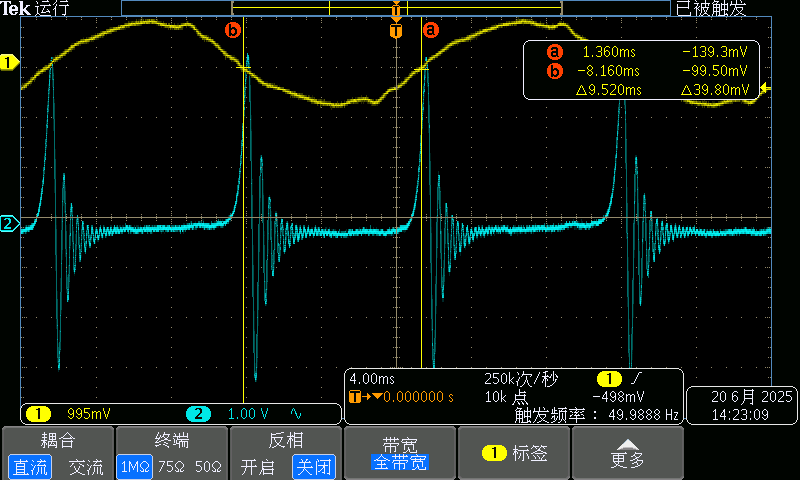
\includegraphics[width=\textwidth]{tek0000_c.png}
        \caption*{硫酸铜水溶液样品1}
    \end{minipage}
    \hfill
    \begin{minipage}[b]{0.32\textwidth}
        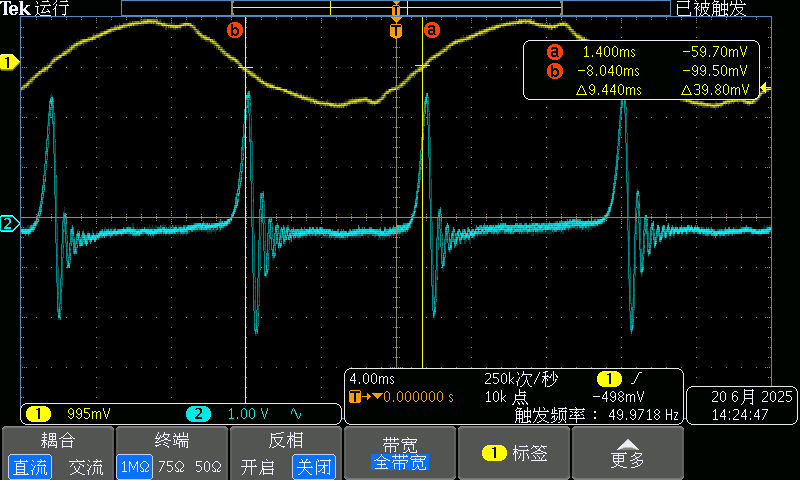
\includegraphics[width=\textwidth]{tek0001_c.png}
        \caption*{硫酸铜水溶液样品2}
    \end{minipage}
    \hfill
    \begin{minipage}[b]{0.32\textwidth}
        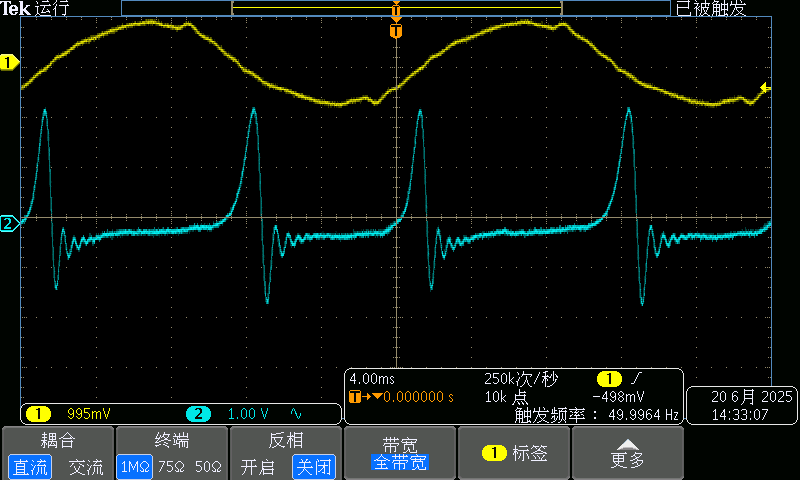
\includegraphics[width=\textwidth]{tek0002_c.png}
        \caption*{硫酸铜水溶液样品3}
    \end{minipage}
    % 第二排：两张图片并排
    \vskip\baselineskip
    \begin{minipage}[b]{0.48\textwidth}
        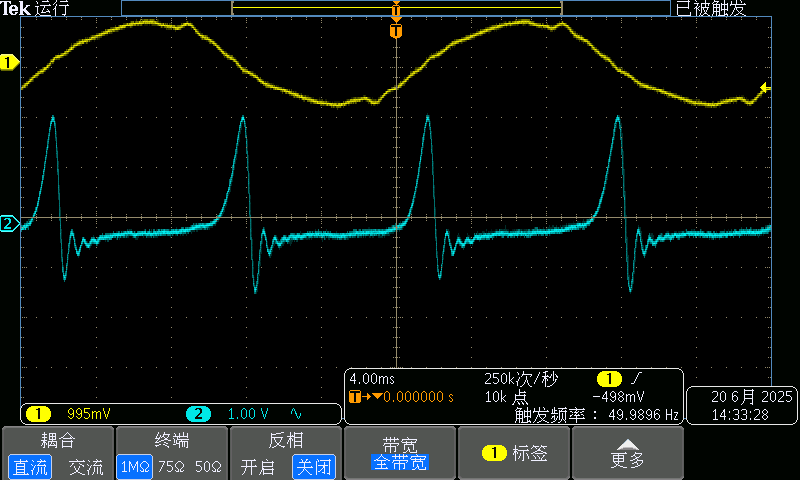
\includegraphics[width=\textwidth]{tek0003_c.png}
        \caption*{硫酸铜水溶液样品4}
    \end{minipage}
    \hfill
    \begin{minipage}[b]{0.48\textwidth}
        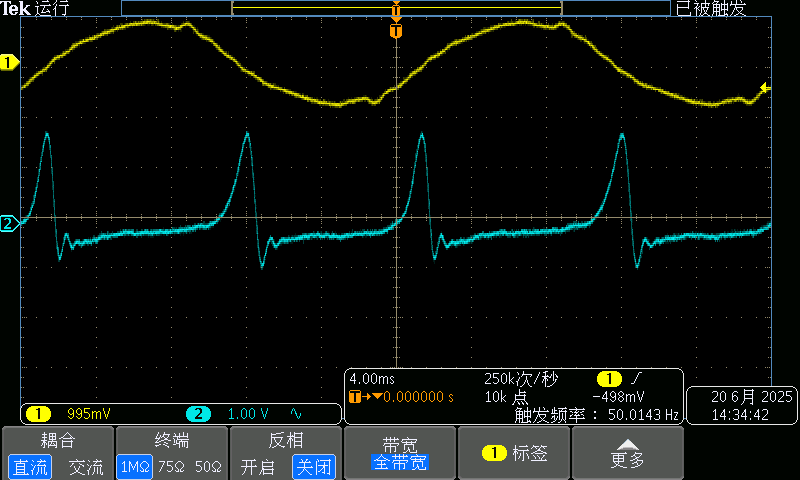
\includegraphics[width=\textwidth]{tek0004_c.png}
        \caption*{硫酸铜水溶液样品5}
    \end{minipage}
    \caption{不同浓度硫酸铜水溶液的共振信号}
    \label{fig:copper}
\end{figure}

从图中我们可以看出，随着浓度的增大，共振信号的弛豫时间逐渐变短。
由实验原理我们可以知道，由于原子核的磁矩在数量级上小于电子的轨道磁矩，共振信号的观察要求样品中所有的氢原子核都处于同步的共振状态。
在共振信号的弛豫过程中，原子核的共振频率会逐渐偏离共振频率。
在样品的浓度较小的时候，对应参与共振的原子核的数量也较少，于是在弛豫的过程中失去同步相位的速度较慢。
而当样品浓度较大的时候，参与共振的原子核数量较多，在弛豫的过程中很快便失去同步相位，混乱的磁矩相位导致平均效应，使得对外表现出来的总磁矩接近于零。
这便会使得共振信号快速衰减，共振信号的弛豫时间变短。

\clearpage
\subsubsection*{旋磁比计算}
按照实验要求，我们使用频率计测出来的共振频率和使用高斯计测出来的磁场强度，计算出旋磁比和g因子。

首先我们给出旋磁比的计算公式
\begin{equation}
    \gamma = \frac{\omega_0}{B_0}
\end{equation}
其中$\omega_0$为共振频率，$B_0$为磁场强度。

我们根据六个样品计算出旋磁比，并和实验室给出的参考数据进行对比，结果如表\ref{tab:gamma}所示。
参考值：$\gamma = 267.52\mathrm{M~rad/s/T}$

\begin{table}[h!]
    \centering
    \begin{tabular}{|c|c|c|}
        \hline
        样品编号 & 旋磁比$(M~rad/T)$ & 相对误差$(\%)$ \\
        \hline\hline
        1 & 299.71 & 11.29 \\
        2 & 299.72 & 11.29 \\
        3 & 299.69 & 11.28 \\
        4 & 299.72 & 11.29 \\
        5 & 299.72 & 11.29 \\
        6 & 299.74 & 11.30 \\
        \hline
    \end{tabular}
    \caption{旋磁比计算结果}
    \label{tab:gamma}
\end{table}

可见我们测出的旋磁比和参考值的相对误差在$11\%$左右，在一定程度上是可以接受的。
不过实验数据整体呈现出偏大的趋势，我们会在后续的误差分析中进行讨论。

\subsubsection*{误差分析}
在本实验中，测量旋磁比的误差主要来源于以下几个方面：
\begin{itemize}
    \item \textbf{磁场强度$B_0$的测量误差}：磁场强度通常通过高斯计测量，受限于高斯计的精度、零点漂移以及探头放置位置的影响，实际测得的磁场值可能与真实值存在一定偏差。
    此外，磁场在空间分布上可能存在不均匀性，样品实际受到的磁场与测量点的磁场可能略有不同。

    \item \textbf{共振频率$\omega_0$的测量误差}：共振频率的测量依赖于频率计的精度以及信号的清晰程度。
    当共振信号较弱或噪声较大时，频率计读数可能不够准确，导致频率测量存在误差。

    \item \textbf{样品定位与均匀性}：样品在磁场中的位置如果发生偏移，或者样品本身分布不均匀，会导致实际参与共振的原子核所处的磁场与测量值不一致，从而影响旋磁比的计算。
    
    \item \textbf{环境因素}：如外部磁场干扰、温度变化等也可能对实验结果产生影响。
\end{itemize}

综上所述，虽然本实验测得的旋磁比与参考值存在约$11\%$的相对误差，但考虑到上述各种误差来源，这一结果在实验允许的范围内是可以接受的。
若要进一步减小误差，可以采用更高精度的仪器、优化样品定位、加强磁场屏蔽等措施。


\subsection*{【思考题】}
由于这个实验的实验讲义中并没有直接给出思考题，我将在这个部分思考并总结我在实验中遇到的一些问题。

\subsubsection*{1.如何测量纯水样片的弛豫时间}
测量纯水样品的弛豫时间（$T_2$ 或 $T_1$）在本实验中具有一定的挑战性，主要原因有以下几点：

1. \textbf{信号“拍”现象的影响}：如前文所述，纯水样品的共振信号呈现出明显的“拍”形状，这种现象会导致信号包络的衰减速度与实际的弛豫过程不完全一致。直接用“拍”信号的包络衰减时间作为弛豫时间，往往会低估真实的$T_2$。

2. \textbf{弛豫时间较长，超出仪器观测范围}：纯水的弛豫时间通常较长（文献值约为$2\,\mathrm{s}$），而实验中示波器的时间窗口有限，难以完整记录信号的全部衰减过程。这会导致测量结果偏小。

3. \textbf{信噪比问题}：纯水的核磁共振信号本身较弱，且弛豫时间长时信号衰减缓慢，后期信号易被噪声淹没，进一步增加了测量难度。

\textbf{改进的测量方法建议：}
\begin{itemize}
    \item \textbf{延长示波器采样时间}：尽量将示波器的时间基线调长，覆盖更长的信号衰减过程，以便更准确地拟合信号包络的指数衰减部分。
    \item \textbf{多次平均}：通过多次重复实验并对信号进行平均，可以提高信噪比，使得信号衰减曲线更加平滑，便于后续数据处理。
    \item \textbf{数据拟合}：将采集到的信号包络用指数函数进行拟合，提取弛豫时间参数。对于“拍”信号，可以先对包络进行包络提取，再进行指数拟合。
    \item \textbf{采用脉冲核磁共振法}：如果实验条件允许，采用脉冲核磁共振（如自旋回波法）可以更准确地测量$T_2$，并有效消除磁场不均匀性带来的影响。
\end{itemize}

\textbf{实验中实际操作：}本实验中，我们采用了延长示波器时间基线和多次平均的方法，尽量捕捉到完整的信号衰减过程。对于“拍”信号，我们提取其包络线并进行指数拟合，得到一个近似的弛豫时间。需要注意的是，这一结果可能仍低于真实的$T_2$，但在实验条件限制下已是较为合理的估算。

\textbf{结论：}测量纯水样品的弛豫时间时，应充分考虑信号“拍”现象和仪器观测范围的影响，采用合适的数据处理和拟合方法，才能获得较为准确的结果。

\subsubsection*{2.如何进行尾波拟合并获得更好的尾波分析}
在核磁共振实验中，尾波（即自由感应衰减信号，FID）的分析对于提取样品的弛豫时间、共振频率等物理参数至关重要。为了获得更好的尾波分析结果，通常需要对实验数据进行合理的拟合处理。以下是尾波拟合的常用方法及改进建议：

\textbf{1. 尾波信号的数学模型}

理想情况下，FID信号可以表示为：
\[
S(t) = A \, e^{-t/T_2} \cos(\omega_0 t + \phi) + C
\]
其中$A$为初始幅度，$T_2$为横向弛豫时间，$\omega_0$为共振角频率，$\phi$为初始相位，$C$为基线偏移。

\textbf{2. 拟合步骤与技巧}

\begin{itemize}
    \item \textbf{数据预处理}：首先应对原始数据进行去噪、去除直流分量（基线校正）等预处理操作。可以采用移动平均、低通滤波等方法提升信噪比。
    \item \textbf{包络提取}：若尾波信号存在“拍”或调制现象，可先通过Hilbert变换或取信号绝对值并平滑，提取信号包络，再对包络进行指数衰减拟合。
    \item \textbf{非线性最小二乘拟合}：利用如Levenberg-Marquardt等非线性拟合算法，对上述模型进行参数拟合，提取$T_2$、$\omega_0$等参数。常用工具有Origin、MATLAB、Python的scipy库等。
    \item \textbf{选取合适的拟合区间}：应避开信号初始的激励脉冲干扰和后期噪声主导的区间，选取信号衰减明显且信噪比较高的部分进行拟合。
    \item \textbf{多次测量与平均}：重复实验多次，取平均结果，可以有效抑制偶然误差，提高拟合的可靠性。
\end{itemize}

\textbf{3. 改进建议}

\begin{itemize}
    \item \textbf{提升采样率和采样精度}：高采样率有助于更准确地还原尾波细节，避免混叠失真。
    \item \textbf{优化实验参数}：如适当调整射频脉冲宽度、幅度，优化样品位置，提升信号强度。
    \item \textbf{采用频域分析}：对尾波信号进行傅里叶变换，分析其频谱结构，有助于识别多组分信号或“拍”现象的成因。
    \item \textbf{利用专业软件}：如MATLAB、Origin、Python等，编写自定义拟合程序，灵活处理复杂信号。
\end{itemize}

\textbf{4. 实验中实际操作举例}

在本实验中，我们采用了以下步骤进行尾波拟合：
\begin{enumerate}
    \item 用示波器记录尾波信号，导出数据。
    \item 用Python对数据进行基线校正和去噪处理。
    \item 对信号包络进行提取，并用指数衰减模型进行拟合，获得$T_2$。
    \item 对于存在“拍”现象的信号，先用Hilbert变换提取包络，再拟合。
    \item 多次测量并取平均，减小偶然误差。
\end{enumerate}

\textbf{结论}：通过合理的数据预处理、包络提取、非线性拟合等方法，可以有效提高尾波分析的准确性和可靠性。若实验条件允许，建议结合频域分析和多次测量，进一步提升结果的可信度。


\bibliography{ref.bib} %biblatex -> 'xelatex->pdfletax->xelatex'
\bibliographystyle{ieeetr}

\subsection*{【原始数据的记录】}
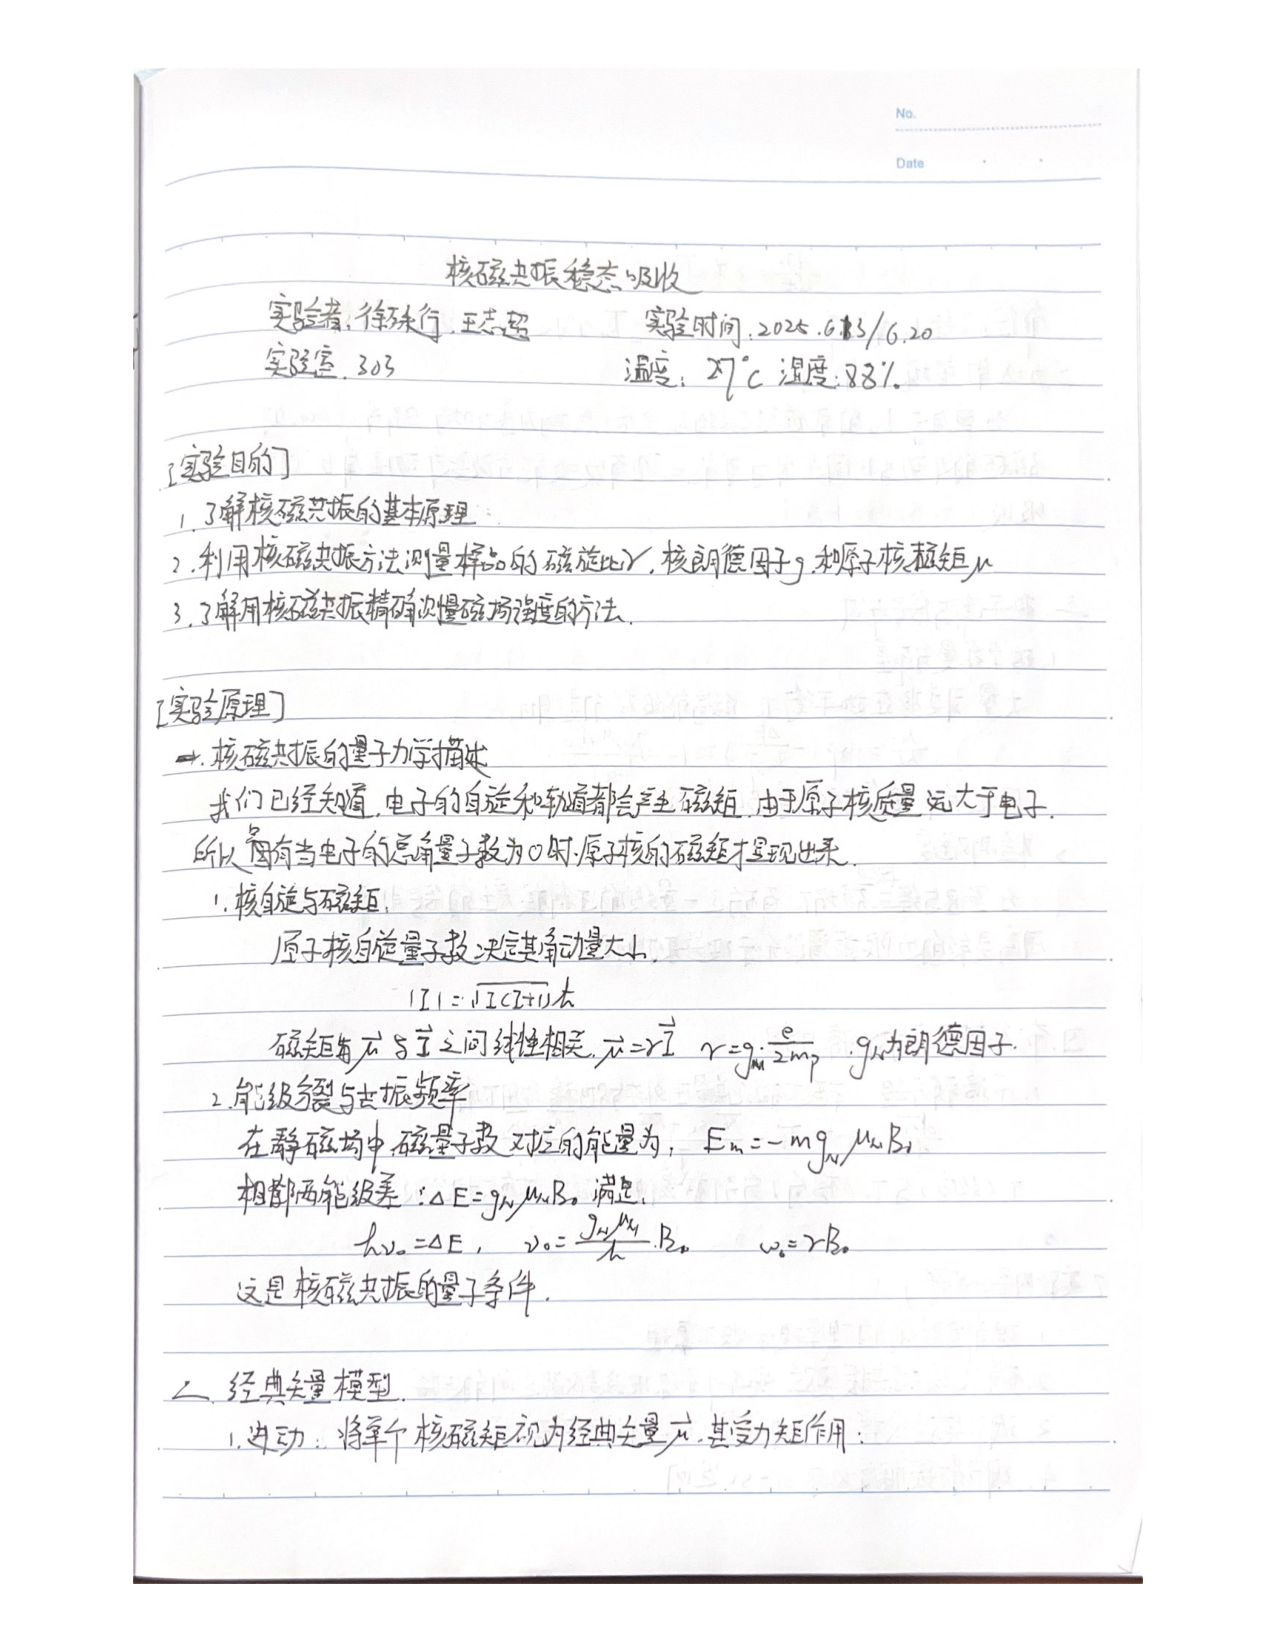
\includepdf[pages=-]{核磁共振scan.pdf}

\end{document}